% Vimtex is great, but damn, running LaTeX locally is such a pain

\documentclass[conference]{IEEEtran}
% \IEEEoverridecommandlockouts
% The preceding line is only needed to identify funding in the first footnote. If that is unneeded, please comment it out.
% \usepackage{cite}
\usepackage[portuguese]{babel}
\usepackage{amsmath,amssymb,amsfonts}
\usepackage{algorithmic}
\usepackage{graphicx}
\usepackage{textcomp}
\usepackage{xcolor}
\usepackage[breaklinks]{hyperref}
\usepackage{microtype}
\usepackage{natbib}
\usepackage{listings}

\def\BibTeX{{\rm B\kern-.05em{\sc i\kern-.025em b}\kern-.08em
    T\kern-.1667em\lower.7ex\hbox{E}\kern-.125emX}}
\begin{document}

\title{Implementação e Ataque da Cifra de Vigenère}

\author{\IEEEauthorblockN{Leonardo Alves Riether}
\IEEEauthorblockA{\textit{Dep. Ciência da Computação} \\
\textit{Universidade de Brasilia}\\
Brasília, Brasil \\
190032413@aluno.unb.br}
}

\maketitle

\begin{abstract}
    If you're reading this I forgot to write an abstract
\end{abstract}

\begin{IEEEkeywords}
    cifra, Vigenère, criptografia, xor
\end{IEEEkeywords}

\section{Introdução} % {{{
Uma maneira simples de cifrar uma mensagem é utilizar a cifra de Vigenère, que
foi criada em 1553 por Giovan Battista Bellaso, e só foi quebrada em 1863. O
método consiste, tradicionalmente, em sobrepor uma mensagem com uma chave
repetida diversas vezes (até que o tamanho da chave se iguale ao da mensagem) e
somar os valores das letras sobrepostas módulo 26.

Neste trabalho, foi desenvolvido um programa que possibilita a cifração e
decifração de uma mensagem com uma cifra de Vigenère modificada, que é
descrito na seção \ref{sec:implementation}. Além disso, é descrito um método de
ataque à cifra, que tenta automaticamente descobrir a chave com a qual um texto
foi cifrado, na seção \ref{sec:attack}.

% }}}

\section{Estruturação do Projeto} % {{{
Neste trabalho, foi implementado um codificador e decodificador da cifra de
Vigenère em C++. O projeto foi compilado com GCC 12.1.0 e testado em Linux , mas
em princípio pode ser compilado em qualquer sistema com GCC que suporte C++17 e
executado tanto em sistemas baseados em Unix quanto no Windows. 

O projeto foi dividido em três partes:

\begin{enumerate}
    \item \textbf{main:} onde estão implementadas as funcionalidades de cifração
        e decifração da cifra de Vigenère, dada uma chave (ou arquivo de chave).
        Esse módulo é explicado na seção \ref{sec:implementation} e pode ser
        compilado com o comando \verb|make main|.
    \item \textbf{findkey:} onde está implementada a função de ataque da
        cifra de Vigenère, que encontra uma chave automaticamente, dada uma
        mensagem cifrada. Esse módulo é explicado na seção \ref{sec:attack} e
        pode ser compilado com o comando \verb|make findkey|. 
    \item \textbf{test:} possui alguns, poucos, testes, que podem ser executados
        com o comando \verb|make test|.
\end{enumerate}

Os comandos \verb|make| geram executáveis dentro do diretório \verb|bin|, por
exemplo \verb|bin/main| e \verb|bin/findkey|. Instruções mais detalhadas para a
execução do \verb|main| e \verb|findkey| podem ser encontradas nas seções
\ref{sec:exec-main} e \ref{sec:exec-attack}, respectivamente.  

Os principais arquivos a serem analisados são os seguintes:
\begin{itemize}
    \item \textbf{main.cpp}: a maior parte desse arquivo é boilerplate para
        chamar as funções de cifração e decifração do módulo \textbf{main}.
    \item \textbf{vigenere.cpp}: possui a implementação das funções de cifração
        e decifração.
    \item \textbf{findkey.cpp}: onde está implementada a função de ataque à
        cifra.
    \item \textbf{scoring.cpp}: possui tabelas de pontuação, que serão
        explicadas na seção \ref{sec:attack}.
\end{itemize}

% }}}

\section{Implementação} % {{{
\label{sec:implementation}

\subsection{Operação de Combinação da Mensagem com a Chave}
Tradicionalmente, na cifra de Vigenère cada letra da mensagem é "combinada" com
uma da chave, por meio da soma módulo 26 dos valores das letras (geralmente, o
valor de A é 0, o de B é 1, e assim por diante). Essa abordagem é interessante
quando se deseja cifrar texto, por sua simplicidade de implementação. No
entanto, existem algumas desvantagems:

\begin{itemize}
    \item Espaços e pontuação não são cifrados, portanto é fácil descobrir o tamanho de cada
        palavra.
    \item É mais difícil cifrar imagens, vídeos e arquivos binários que existem
        hoje em dia.
    \item Existem apenas 26 possibilidades para cada letra da mensagem
\end{itemize}

Dado isso, neste trabalho foi implementada uma variação da cifra de Vigenère
tradicional, que utiliza a operação de \textbf{xor bit-a-bit} entre cada byte da mensagem
e da chave. Com isso, é mais difícil descobrir o tamanho das palavras de um
texto cifrado, é possível cifrar qualquer tipo de arquivo, e existem 256
possibilidades para cada byte da chave, tornando essa cifra um pouco mais
difícil de quebrar.

\subsection{Codificação em Base 64}
\label{sec:base64}
Uma desvantagem de utilizar o xor é que o arquivo cifrado pode conter caracteres
ilegíveis. Para manter uma certa compatibilidade com a cifra de Vigenère
implementada com soma módulo 26, foi implementado um codificador e decodificador
de base 64. Os arquivos cifrados e codificados em base 64 utilizam apenas
caracteres legíveis, em troca de um aumento de aproximadamente 33\% do tamanho
do arquivo.

\subsection{Execução do Programa}
\label{sec:exec-main}
Após compilação do programa com \verb|make main|, é possível executá-lo com
alguns argumentos de linha de comando:

\begin{itemize}
    \item \textbf{-k} \textbf{--key}: Especifica uma string que será usada como
        chave da cifra.
    \item \textbf{-kf} \textbf{--key-file}: Espefifica um arquivo cujo conteúdo
        será usado como chave.
    \item \textbf{-i} \textbf{--input}: Determina qual o arquivo de mensagem (ou
        input). Se essa opção não for especificada, é utilizada a entrada padrão
        (stdin).
    \item \textbf{-o} \textbf{--output}: Determina qual o arquivo de cifra (ou
        output). Se essa opção não for especificada, é utilizada a saída padrão
        (stdout).
    \item \textbf{-i64} (\textit{resp.} \textbf{-o64}): Flag que, se usadas,
        indica que a entrada (\textit{resp.} saída) está codificada em base 64.
\end{itemize}

É necessário especificar uma chave, por meio de um argumento \textbf{-k} ou
\textbf{-kf}.

% }}}

\section{Ataque} % {{{
\label{sec:attack}

\subsection{Ideia}
É impossível projetar um ataque "universal" à cifra de Vigenère, visto que uma
mensagem aleatória, quando cifrada com uma chave qualquer, gera texto cifrado
aleatório. Esse caso é semelhante à aplicação de um one time pad
(\cite{one-time-pad}), que é matematicamente "inquebrável", se usado
corretamente.

Apesar disso, se a mensagem tiver alguma propriedade que conhecemos a priori, a
cifra de Vigenère pode ser quebrada. Assim, nessa seção consideraremos que a
mensagem cifrada é um texto relativamente longo, escrito em português ou inglês.
O ataque descrito também se aplica a outras línguas, mas focamos nessas duas.
Duas propriedades importantes de textos em português e inglês são:
\begin{enumerate}
    \item A grande maioria dos bytes é legível, diferentemente de arquivos de
        imagens ou executáveis.
    \item É esperado que as frequências dos caracteres sigam uma distribuição
        similar a outros textos escritos na mesma língua.
\end{enumerate}

Sabendo disso, podemos elaborar uma estratégia para encontrar uma chave
provável, dado um texto cifrado e a informação da língua em que a mensagem foi
escrita. A estratégia consiste no seguinte algoritmo:

\begin{enumerate}
    \item Encontrar os tamanhos mais prováveis para a chave.
    \item Para cada tamanho $K$:
        \begin{enumerate}
            \item Separamos os índices da cifra em classes de equivalência
                módulo $K$.
            \item Para cada classe de equivalência, geramos o byte que produz
                maior pontuação, de acordo com uma tabela de frequências. 
            \item A pontuação para a chave de tamanho $K$ gerada é a soma das
                pontuações de cada classe de equivalência.
        \end{enumerate}
    \item A saída é a chave com maior pontuação
\end{enumerate}

Cada parte desse algoritmo é descrito em mais detalhes nas próximas subseções.  

Observe que uma chave de tamanho $K$ particiona a cifra em $K$ classes de
equivalência, e que cada classe precisa de um número grande de bytes para que o
ataque tenha maior chance de funcionar. Assim, quanto maior a razão entre
tamanho da mensagem e tamanho da chave, maior a probabilidade do ataque ser bem
sucedido.

\subsection{Encontrando Tamanhos de Chave Mais Prováveis}
\label{sec:tamanhos}

Em textos grandes, é bem provável que certas algumas combinações de caracteres
se repitam frequentemente. Por exemplo, em inglês, o trigrama \textit{"the"}
provavelmente aparece muitas vezes. Nas vezes que um trigrama se repete na
mensagem e, por acaso, é cifrado com os mesmos índices da chave, o trigrama
cifrado também se repete!

Utilizamos esse fato para encontrar os tamanhos de chave mais prováveis com um
esquema de pontuação dos tamanhos. Primeiro, computamos a distância entre todas
as repetições de trigramas da cifra. Se uma repetição tem distância $\Delta $,
adicionamos um ponto a todos os divisores de $\Delta $. Por último, ordenamos os
inteiros com base em sua pontuação.

Um detalhe de implementação interessante é o algoritmo usado para encontrar os
divisores de um número. Nesse trabalho, foi utilizado o algoritmo de Pollard-Rho
\cite{pollard-rho}. A implementação foi retirada de \cite{pollard-rho-tiago}.

Esse método é chamado de Eliminação de Kasiski e é explicado em mais detalhes em
\cite{kasiski}.

\subsection{Geração de uma Chave de Tamanho K}
\label{sec:pontuacao}
Por meio da Eliminação de Kasiski, obtemos uma lista de tamanhos prováveis para
a chave. Agora, veremos como, dado um tamanho de chave $K$, obter a ``melhor``
chave com tamanho $K$. Para determinar qual chave é ``melhor`` ou ``pior``,
definimos uma função de pontuação que recebe uma chave e atribui a ela um
número. Quanto mais provável a chave, maior deve ser sua pontuação. 

Nesse ponto, notamos que, para uma chave de tamanho $K$, se dois índices $i, j$ da
mensagem são congruentes módulo $K$, eles foram cifrados com o mesmo byte da
chave. Sendo assim, podemos particionar os índices em classes de equivalência
módulo $K$ e encontrar cada byte da chave separadamente.

Um modo de encontrar um byte da chave para uma classe de equivalência é testar
todas as possibilidades para o byte e comparar as tabelas de frequências com a tabela
esperada da língua. Essa comparação é mais fácil na cifra de Vigenère com soma
módulo 26, porém mais difícil com a cifra baseada em xor bit-a-bit, visto que
teríamos que gerar uma tabela com a frequência de espaços, pontuação e outros
símbolos que podem aparecer na mensagem. Por conta disso, é proposto outro modo
de pontuar a classe, baseada em ideias de \cite{breaking-the-cipher}.

Utilizando as tabelas esperadas de frequência de textos em inglês e português,
mostradas respectivamente em \ref{tab:englishfrequency} e
\ref{tab:portuguesefrequency}, executamos o algoritmo que é mostrado em
pseudocódigo em \ref{code:idk}. A variável \verb|tabela| associa os valores
ascii das letras às suas respectivas frequências na língua adequada, os demais
bytes possuem valor zero na tabela.

Em poucas palavras, esse algoritmo itera pelos possíveis valores de
\verb|chave[i]|, decodifica a cifra com cada valor e pontua com base nos valores
da tabela para os bytes decifrados. Após isso, o byte que produziu o maior score
é escolhido. Como a tabela é baseada na frequência esperada dos caracteres,
espera-se que o caracter real da chave maximize a pontuação.

\begin{table}[htbp]
\caption{Frequência das Letras em Textos escritos em Inglês}
\begin{center}
\begin{tabular}{|c|c|c|c|}
\hline
    Letra & Frequência & Letra & Frequência \\
\hline
    E & 11.1607\% & M & 3.0129\% \\
    A & 8.4966\% & H & 3.0034\% \\
    R & 7.5809\% & G & 2.4705\% \\
    I & 7.5448\% & B & 2.0720\% \\
    O & 7.1635\% & F & 1.8121\% \\
    T & 6.9509\% & Y & 1.7779\% \\
    N & 6.6544\% & W & 1.2899\% \\
    S & 5.7351\% & K & 1.1016\% \\
    L & 5.4893\% & V & 1.0074\% \\
    C & 4.5388\% & X & 0.2902\% \\
    U & 3.6308\% & Z & 0.2722\% \\
    D & 3.3844\% & J & 0.1965\% \\
    P & 3.1671\% & Q & 0.1962\% \\
\hline
\end{tabular}
\label{tab:englishfrequency}
\end{center}
\end{table}

\begin{table}[htbp]
\caption{Frequência das Letras em Textos escritos em Português}
\begin{center}
\begin{tabular}{|c|c|c|c|}
\hline
    Letra & Frequência & Letra & Frequência \\
\hline
    A & 14.63\% & B & 1.04\% \\
    C & 3.88\% & D & 4.99\% \\
    E & 12.57\% & F & 1.02\% \\
    G & 1.30\% & H & 1.28\% \\
    I & 6.18\% & J & 0.40\% \\
    K & 0.02\% & L & 2.78\% \\
    M & 4.74\% & N & 5.05\% \\
    O & 10.73\% & P & 2.52\% \\
    Q & 1.20\% & R & 6.53\% \\
    S & 7.81\% & T & 4.34\% \\
    U & 4.63\% & V & 1.67\% \\
    W & 0.01\% & X & 0.21\% \\
    Y & 0.01\% & Z & 0.47\% \\
\hline
\end{tabular}
\label{tab:portuguesefrequency}
\end{center}
\end{table}

\begin{lstlisting}[language=Python, caption=Cálculo da pontuação para um tamanho
de chave K]
# K = tamanho da chave
# M = tamanho da mensagem
for i in range(K): # classe de equivalencia
  score = [0] * 256 # lista com 256 zeros
  for x in range(256):
    for j in range(i, M, K):
      # (^) representa o xor bit-a-bit
      score[x] += tabela[mensagem[j] ^ x]
  chave[i] = max_index(score)
\end{lstlisting}
\label{code:idk}

\subsection{Escolha da Chave Mais Provável}
\label{sec:escolha}
Após a geração de várias chaves com tamanhos diferentes, cada uma terá uma
pontuação, que é dada pela soma das pontuações de cada um de seus bytes. Com
isso, podemos dizer que a chave com maior pontuação total é a mais provável, e
será a saída do programa de ataque desenvolvido. 

\subsection{Execução do Programa de Ataque}
\label{sec:exec-attack}

Após compilação do programa de ataque com \verb|make findkey|, é possível
executar \verb|bin/findkey| com alguns argumentos de linha de comando:

\begin{itemize}
    \item \textbf{-i} \textbf{--input}: arquivo de entrada cifrado.
    \item \textbf{-o} \textbf{--output}: arquivo de saída, que conterá a chave
        gerada.
    \item \textbf{-l} \textbf{--lengths}: determina a quantidade de tamanhos de
        chaves testados.
    \item \textbf{-min} (\textit{resp.} \textbf{-max}): tamanho mínimo (
        \textit{resp.} máximo) das chaves a serem testadas.
    \item \textbf{--english} ou \textbf{--portuguese}: indicam qual tabela de
        frequências deve ser utilizada para pontuar as chaves.
\end{itemize}

Um exemplo da execução da cifração, seguido de um ataque, e por último
decifração utilizando a chave prevista pelo ataque, é mostrada na figura
\ref{fig:example}.

\begin{figure}[htbp]
    \centerline{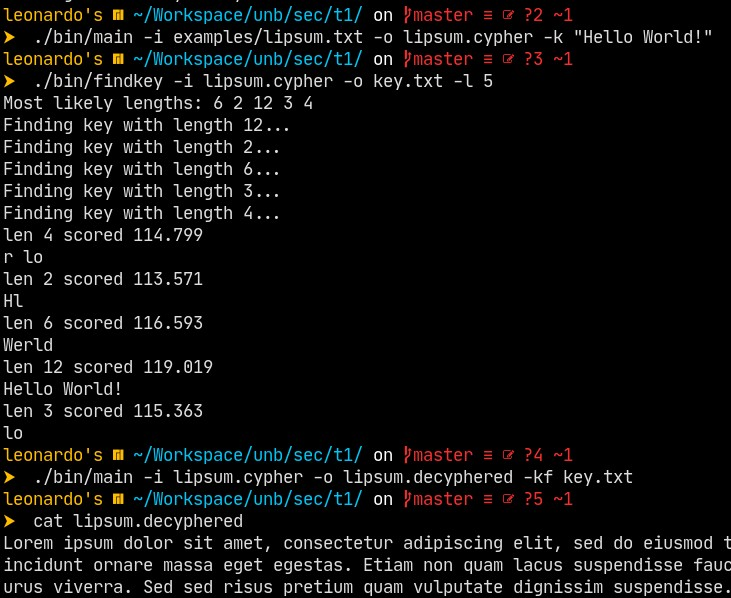
\includegraphics[width=\linewidth]{img/ss1.jpg}}
\caption{Exemplo de Execução}
\label{fig:example}
\end{figure}

% }}}

\section{Conclusão} % {{{
\label{sec:conclusion}

% }}}

% \begin{table}[htbp]
% \caption{Table Type Styles}
% \begin{center}
% \begin{tabular}{|c|c|c|c|}
% \hline
% \textbf{Table}&\multicolumn{3}{|c|}{\textbf{Table Column Head}} \\
% \cline{2-4} 
% \textbf{Head} & \textbf{\textit{Table column subhead}}& \textbf{\teu conseextit{Subhead}}& \textbf{\textit{Subhead}} \\
% \hline
% copy& More table copy$^{\mathrm{a}}$& &  \\
% \hline
% \multicolumn{4}{l}{$^{\mathrm{a}}$Sample of a Table footnote.}
% \end{tabular}
% \label{tab1}
% \end{center}
% \end{table}

% \bibliographystyle{IEEEtran}
\bibliographystyle{unsrtnat}
\bibliography{bib}

\end{document}

